\documentclass[aps,onecolumn,12pt,letterpaper,amsmath,amssymb,floatfix,pra,notitlepage]
{revtex4-1}
\renewcommand{\topfraction}{0.9}
\renewcommand{\textfraction}{0.1}
\usepackage{graphicx}
\usepackage{dcolumn}
\usepackage{bm}
\usepackage{hyperref}
\usepackage{hhline}
\usepackage{cprotect}
\usepackage{titlesec}
\titlespacing*{\section}{0pt}{12pt}{6pt}
\titlespacing*{\subsection}{0pt}{10pt}{4pt}
\topmargin -0.65in
\headsep 20.0pt
\def\theYear{\the\year}
\usepackage{float}
\usepackage{placeins}
\graphicspath{{figures/}}
\begin{document} 

  \setcounter{page}{1}


\title{How our atmosphere obscures planets: a model of the effect of telluric contamination on solar emission lines}

\author{Meltem Acar}

\affiliation{Institute for Computing in Research}

\date{\today}

\maketitle
\vspace{-0.5in}
\section{Abstract}

Ground based telescopes are continuously observing the solar spectrum of distant stars, which they are doing so to extract data and calculate measurements. These measurements specifically relevant in this paper are radial velocity shift measurements. Whereas observing and calculating radial velocity shift measurements of the wavelengths we observe from stars is used to detect the presence exoplanets orbiting a star. However, when we are trying to measure this light that these stars emit, we come across difficulties with trying to collect data with a ground based telescope rather than a telescope already out in space. Since the light has to pass through Earth's atmosphere, the gasses in our atmosphere such as water vapor and carbon dioxide, selectively absorb light at specific wavelengths. This creates what is known as telluric lines. These telluric lines can interfere when observing spectral lines, as they tend to overlap and create error within observing spectral lines. In this project we want to determine if the location of telluric lines has impacts on how we can calculate the center point of a spectral line, then how the radial velocity shift calculations are impacted from that. The results aim to model a visual representation of how shifting telluric contamination to impact the shape of the spectral line to skew it more or to skew it less. This modeling provides insight on how telluric line position and severity should also be accounted for during radial velocity shift calculations. 


\section{Background}
\subsection{The Doppler Effect}
The Doppler effect is known as the change in observed frequency or wavelength of a wave relative to an observer. If the source approaches the observer, the waves are compressed. As the source moves away from the observer, the waves stretch out. For light waves, this motion of a source creates a change in color. Blueshift; if the source is moving towards the observer, the waves are compressed and are at a higher wavelength. Redshift; if the source is moving away from the observer, the waves are stretched and at a lower wavelength. 

Measuring a stars Doppler shift gives us the ability to determine it's radial velocity. As we receive the wavelengths that a star gives off, not to get confused, the Doppler shift of a star is measured as the change in the wavelength of light. This is the \textit{physical phenomenon} and our \textit{observable data}. The radial velocity however, is the actual speed of a stars wavelength that is either moving towards or away from us, the observer. 

We can use the Doppler shift formula, rearranged, to isolate different variables that we want. In this case, we would isolate the radial velocity variable to calculate it's value. Where \(\Delta\lambda=\) the amount the wavelength has shifted. \(\lambda_\text{0}=\) the original unshifted wavelength. \({V_r}=\) the radial velocity. And \({c}=\) the speed of light.  
$$\frac{\Delta\lambda}{\lambda_{\text{0}}}=\frac{V_r}{c}$$


When a planet orbits a star, it creates a gravitational tug that causes that star to "wobble" back and forth. This wobble is because the planet does not perfectly orbit its stars center, but rather both the star and the planet have a 'shared center of mass', known as the \textit{barycenter}. 

Measuring this periodic shift in a stars spectrum, we are able to calculate the planets mass and other orbital characteristics. This is useful to also detect hidden exoplanets orbiting distant stars. 

\subsection{The Voigt profile}
The Voigt profile is a mathematical curve that describes the shape of spectral lines. It is most commonly used to fit spectral graphs, to find a center point. The Voigt profile itself is created by convolving two different curves, such as the \textit{Gaussian curve} and the \textit{Lorentzian curve}. The Voigt profile is important because it provides a real-world representation of absorption and emission lines. I will be using Pythons "scipy.special.voigt--profile" to model and use it's graph. 

\section{Methods} 
The Voigt profile will be used to model a spectral line, instead of using data from a real spectral line we will be generating modeled data ourselves. We use the Voigt profile to add in varying locations of telluric lines to see how the location and intensity of these telluric lines impact our representation of a spectral line, the Voigt profile. In this case since we are dealing with a very smooth representing spectral line, we can add in these telluric lines and calculate both the center points over time and the radial velocity shift, without having to worry much about any low-level noise. In order to calculate the center point of the Voigt profile, we will use the "Full-Width-Half-Maximum" method. This method is where you take the maximum value of the spectral line, divide that in half to get two width points, where we then divide the width by half again to find our true center line. We repeat this process of finding the center line as we shift the graph along the axis, moving it through our chosen locations and intensity of telluric lines. This is done because light waves are moving as they approach us. To model the "Doppler Effect" on the produced data, we make the Voigt profile "wobble" slightly back and forth as it shifts along the axes. The center line points then are used to calculate the radial velocity shift. Once graphed, we compare the radial velocity shift results of a Voigt profile with three telluric lines at different locations with differing intensity, to another Voigt profile with two telluric lines with similar but greater intensity. *Note: The first two shown graphs are \textit{not to scale} and serves the purpose for visual representation of the Full Width Half Maximum method only. 
\FloatBarrier

\section{Results}

\begin{figure}[!ht]
    \centering
    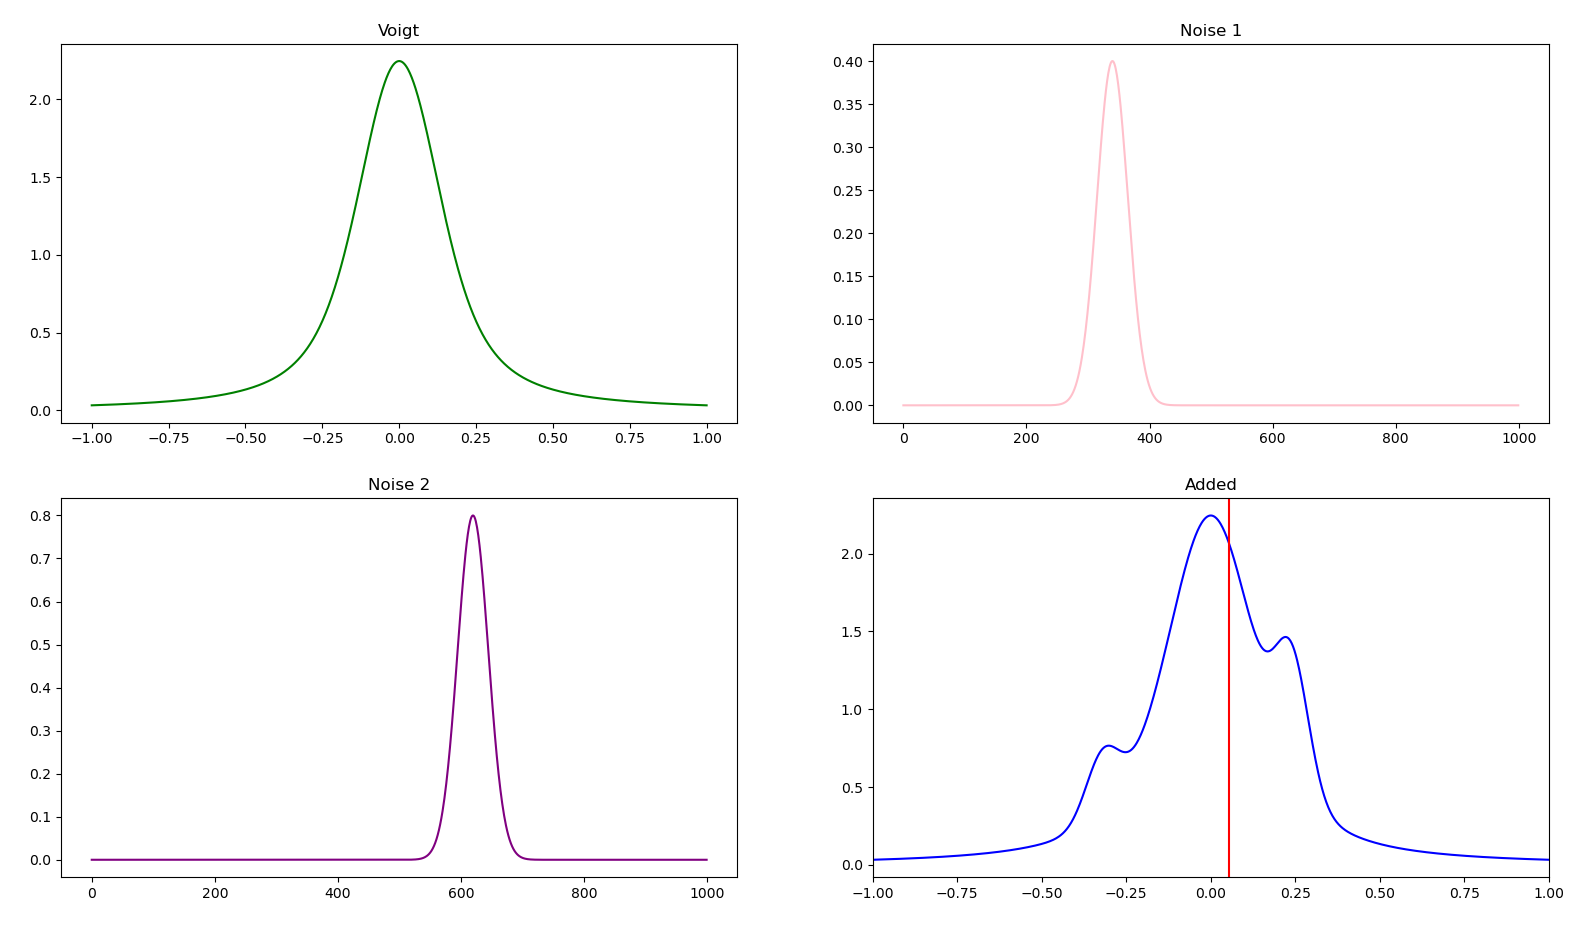
\includegraphics[width=0.8\textwidth]{graphvvv.png}
    \caption{Representation of Voigt profile with and without telluric contamination, along with a visual of where the center point is on the contaminated Voigt profile.}
    \label{fig:voigt2}
\end{figure}
After figuring out the "Full With Half Maximum" method, we are now able to shift the Voigt profile with contamination along the axis. This is done because we want to find the center point over time, which models how a telescope would be taking snapshots and collecting data every minute or so. Which in this model, our "telescope" would be taking snapshots for a time period of around 60 minutes.

\begin{figure}[!ht]
    \centering
    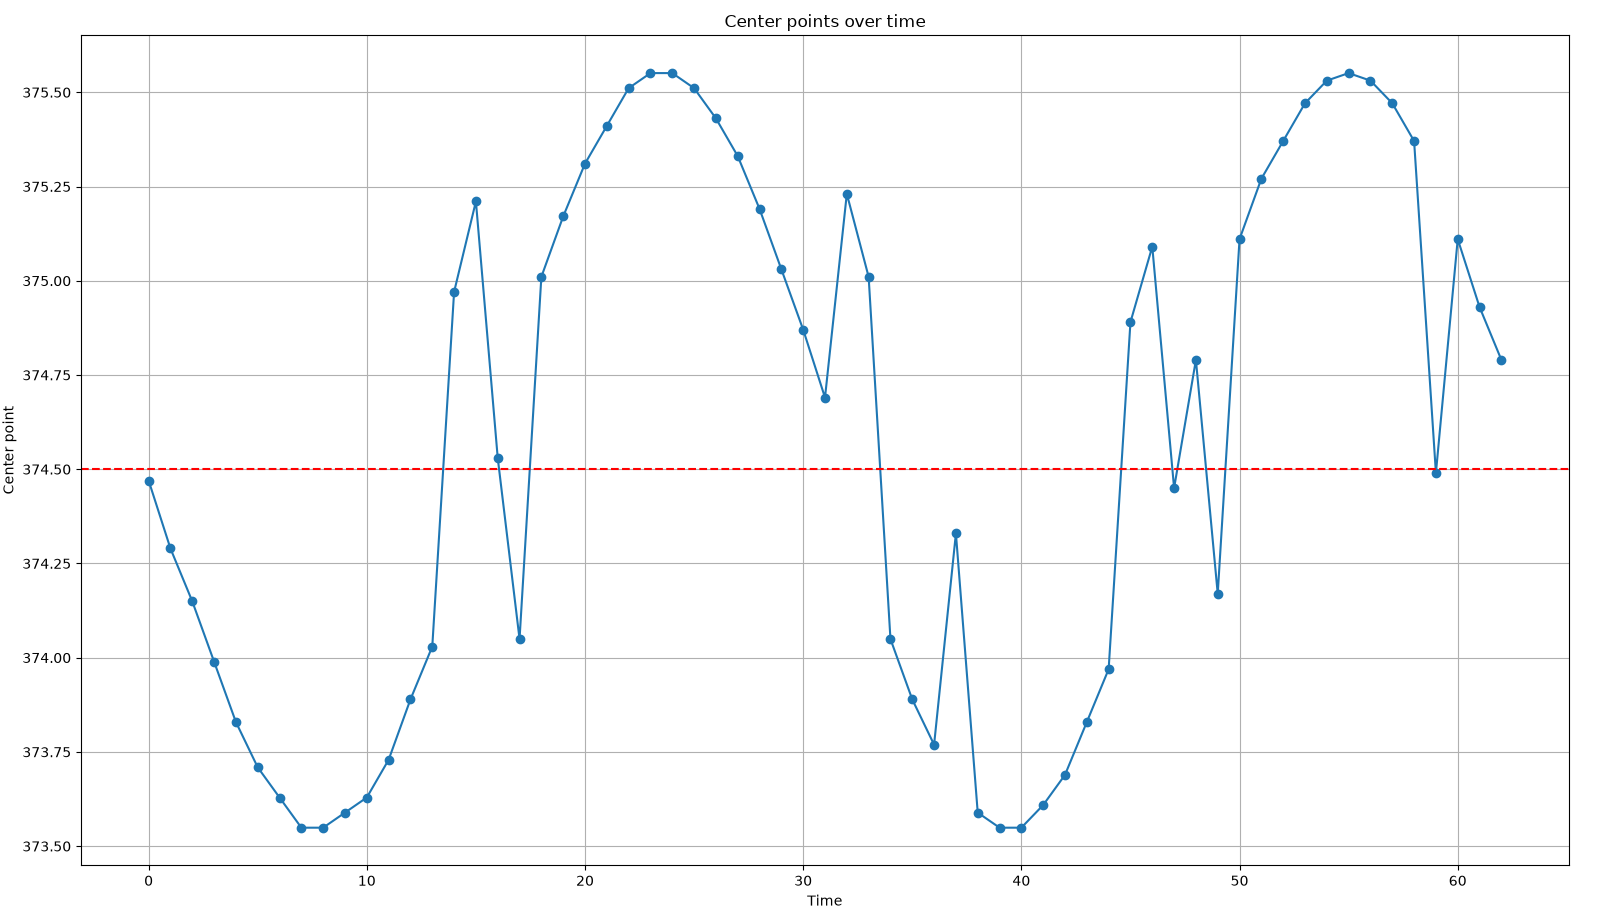
\includegraphics[width=0.8\textwidth]{centerpointsovertime.png}
    \caption{This is a graph of the calculated center points over time of the Voigt profile with 3 telluric lines, one shifted left, two shifted right with where each one has a differing intensity.}
    \label{fig:voigt3}
\end{figure}

\begin{figure}[!ht]
    \centering
    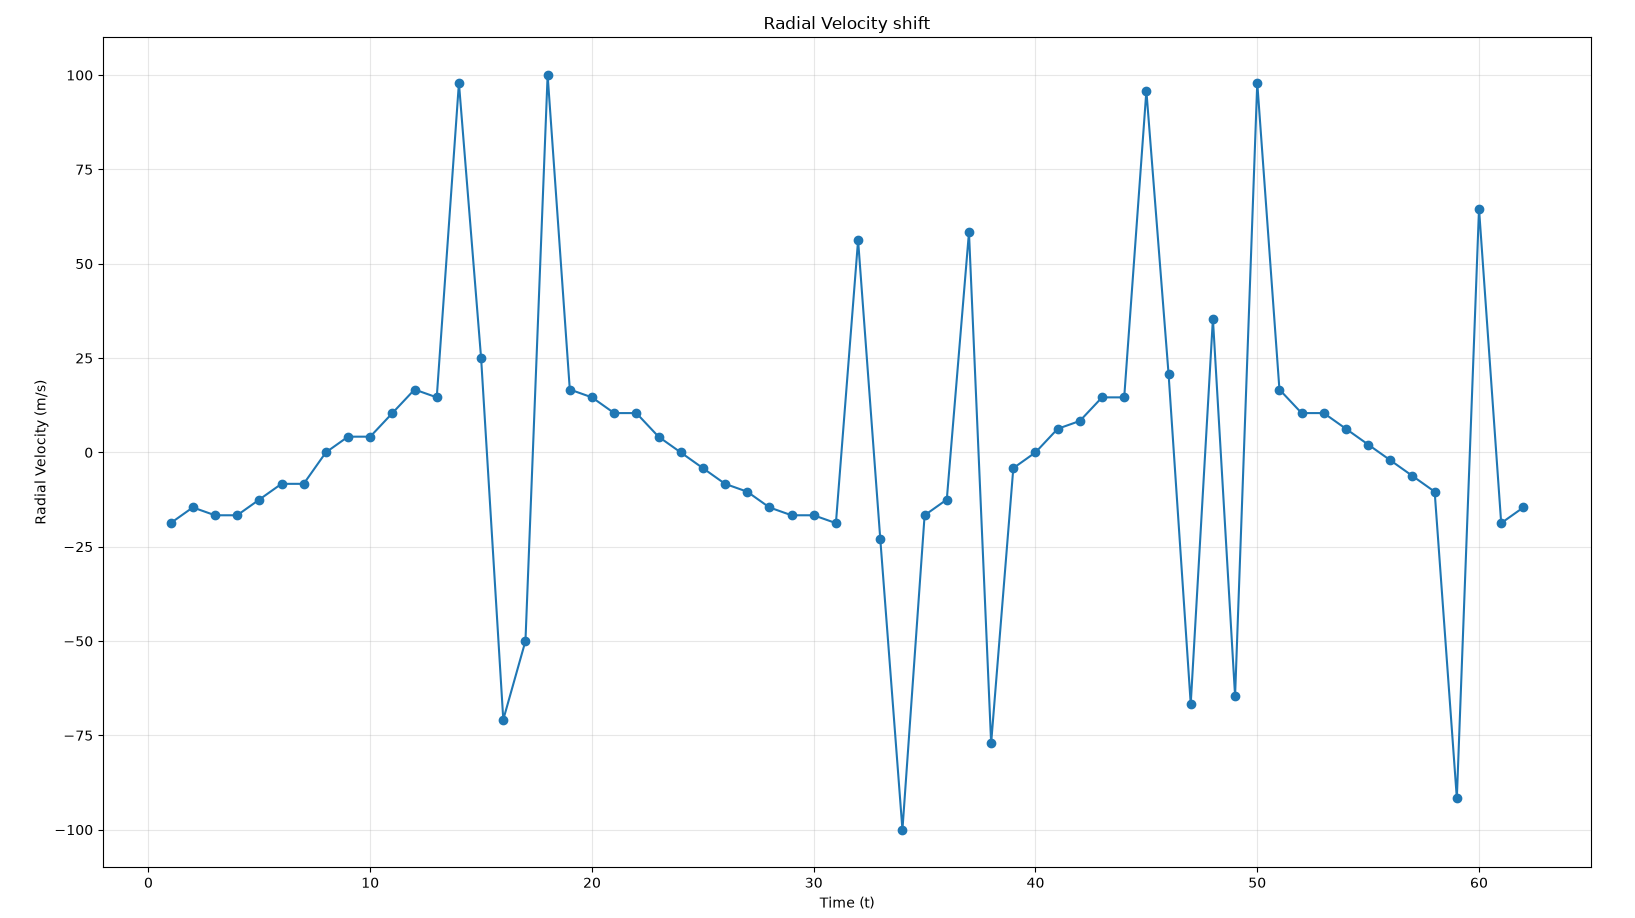
\includegraphics[width=0.8\textwidth]{RVS1.png}
    \caption{This is the graph of the calculated Radial Velocity Shift of the center points in FIG.2.}
    \label{fig:voigt5}
\end{figure}

\begin{figure}[!ht]
    \centering
    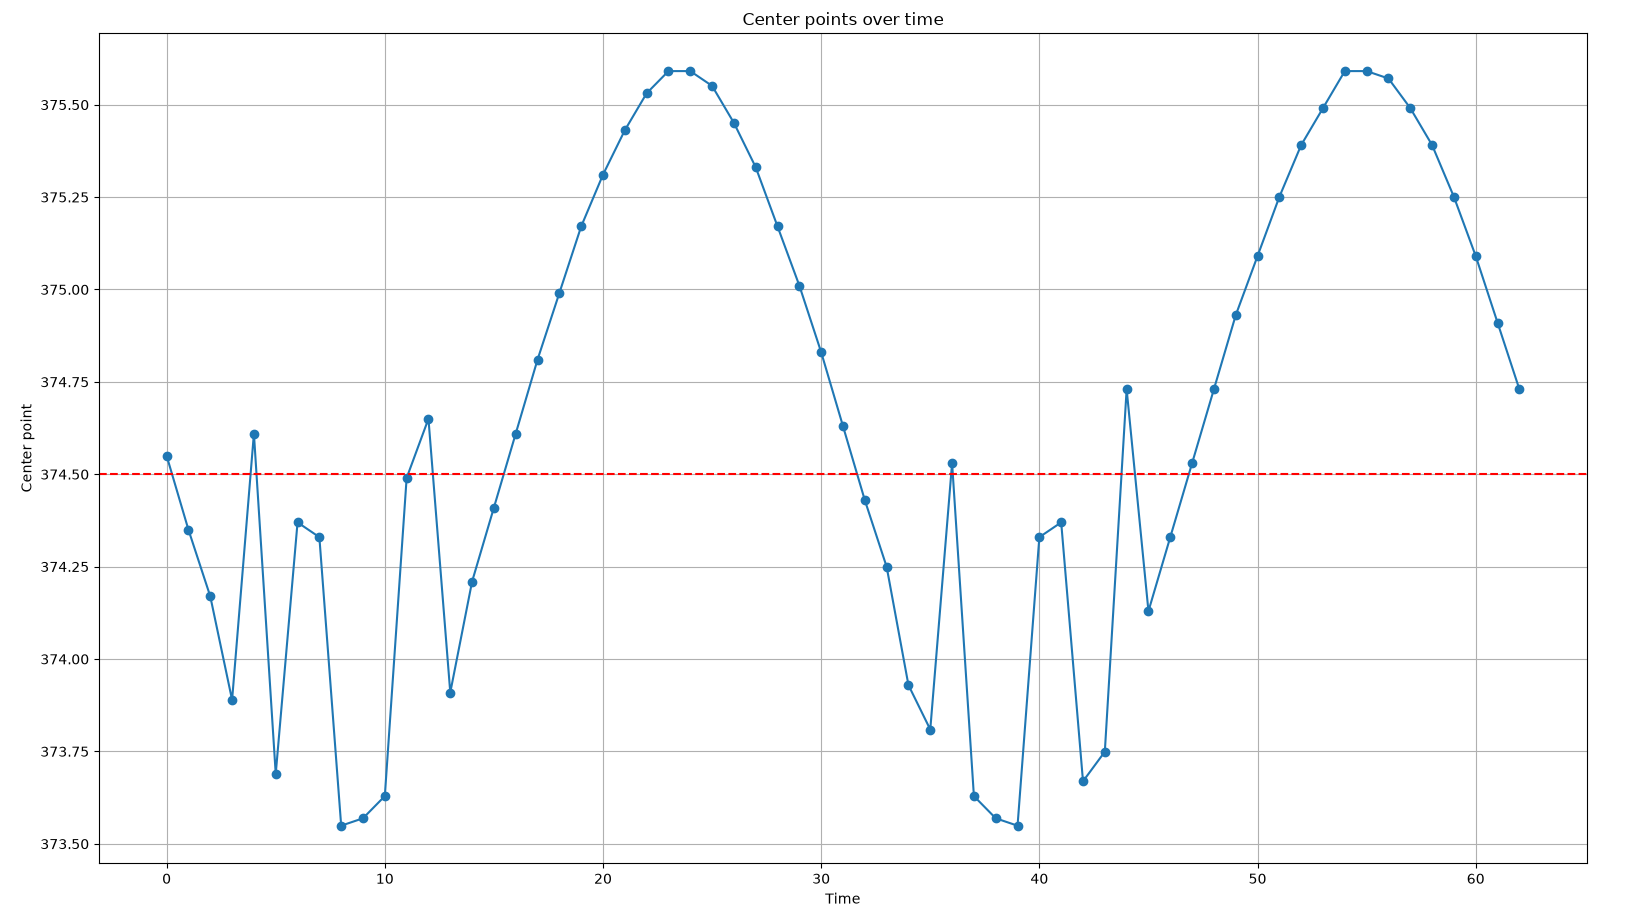
\includegraphics[width=0.8\textwidth]{center2.png}
    \caption{This is another graph of the calculated center points over time of the Voigt profile with 2 telluric lines, at different locations, however the intensity of these telluric lines are much larger.}
    \label{fig:voigt5}
\end{figure}

\begin{figure}[!ht]
    \centering
    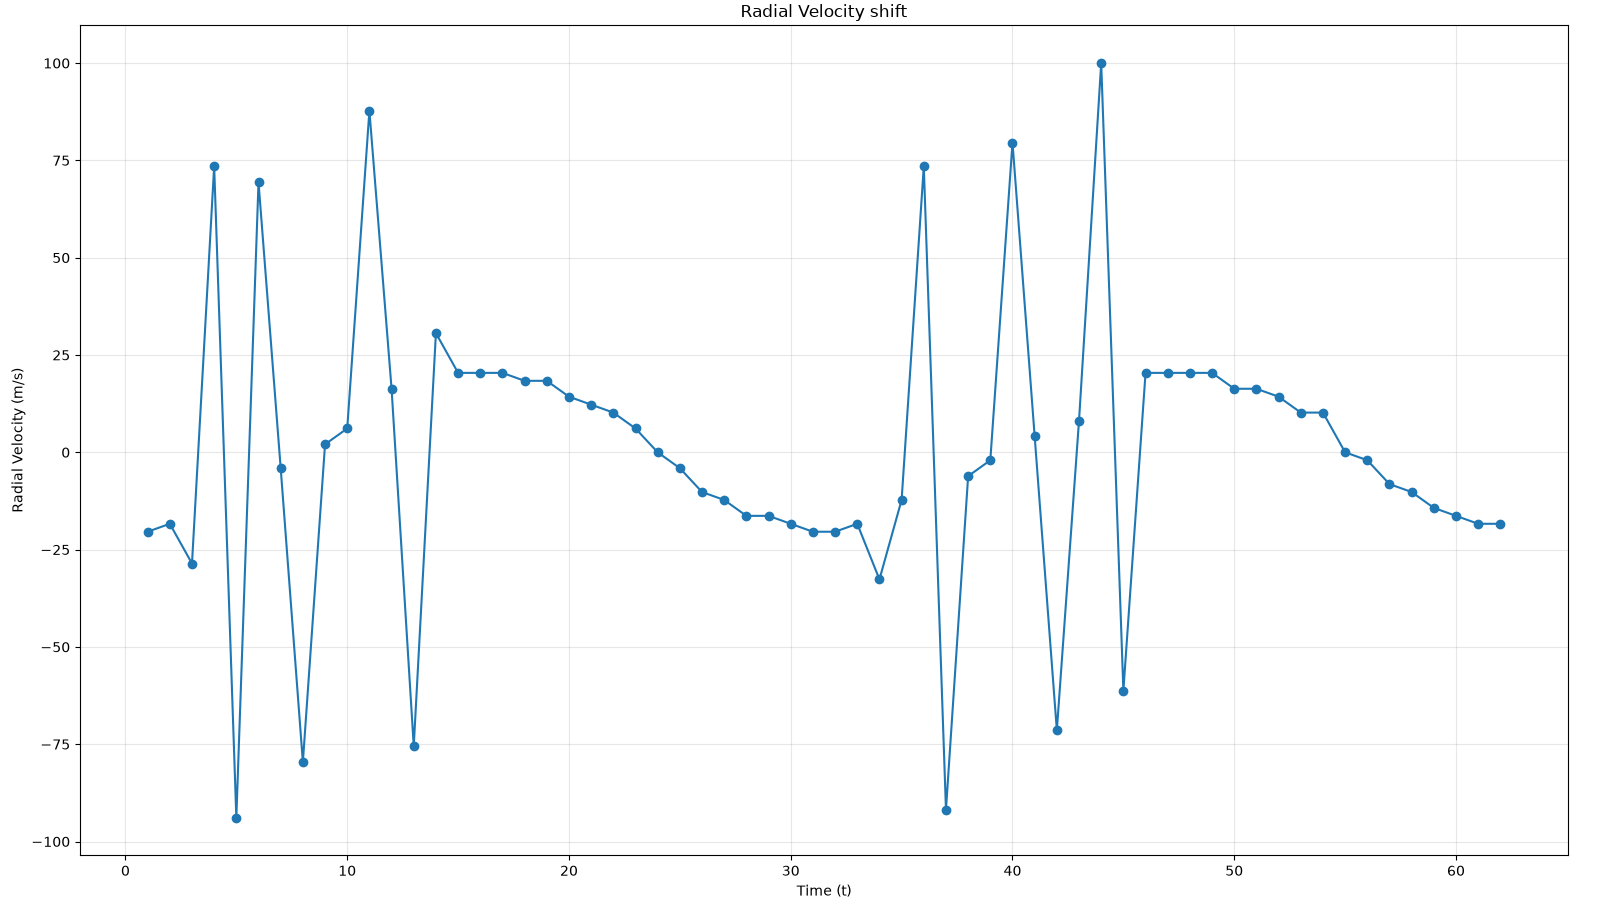
\includegraphics[width=0.8\textwidth]{RVS2.png}
    \caption{This is the graph of the calculated Radial Velocity Shift of FIG.4.}
    \label{fig:voigt5}
\end{figure}

\FloatBarrier

\section{Discussion}
As we observe our given results, we can see that in the two examples modeling telluric contamination in different locations, that if there are more telluric lines, but not as intense present near the Voigt profile as it is shifting, it creates less of an impact then if the telluric lines are fewer but more intense. As a result we can conclude that more intense telluric contamination greatly skews the spectral line shape as it directly overlaps with the spectral line fully. From finding the center points over time, we can also see that when doing the radial velocity shift calculations we come across larger errors, since it is also just very visually prominent where the telluric lines were most impactful on the Voigt profile, because of the visualized large jumps in both of the models of the radial velocity shift calculations. 
\subsection{The relevance}
These results highlight the importance of telluric line identification and removal, particularly for spectral lines which wavelengths happen to fall near strong atmospheric absorption molecules. The removal in telluric lines and studying how their location and intensity is needed, since telluric contamination can create confusion when observing a stars spectrum, where it can cause us to miss the detection of an exoplanet orbiting a star. 

\section{Conclusion} \label{sec:conc}
In this project the effect of telluric contamination on the calculations of center points, and radial velocity shift measurements was modeled by using a representation of the shape of a spectral line, the Voigt profile. By varying the location of telluric lines, and their intensity on the Voigt profile, we were able to observe that the location of contamination significantly affects the accuracy of the calculated radial velocity shift. Overall, this model shows how these results demonstrate that telluric contamination is not a a uniform or constant source of error, but rather one which impact depends strongly on the specific area that it overlaps with on that spectral line. 
For future reference, this model could be extended to be more realistic, with the addition of "low-level noise", which makes finding the center point of the shifting spectral line more challenging. As well as using real data from a star. 


%\section*{Acknowledgements}

%I would like to thank the Institute for Computing in Research, the PDX director Doug Mandell, Mark Galassi, and my mentor who supported me throughout my entire project, Max Kingston. 
\end{document}


 
